\section{Vorgehensmodelle}
(Autor: Dreher)
Wie in Kapitel \ref{sec:einfuehrung} beschrieben, basieren alle Vorgehensmodelle auf wenigen klaren Regeln. Die bedeutendsten Modelle werden in diesem Kapitel genauer erläutert.

\subsection{Extreme Programming}
Extreme Progamming (XP) ist eine der ältesten agilen Vorgehensmodelle und gibt Vorgaben für die Planung, das Management, das Quellcodedesign, das Testmanagement und die Programmierung eines Softwareprojekts. Dadurch wird XP sehr mächtig, aber auch anspruchsvoll für alle Beteiligten. \cite{bib:wolfRoock} \cite{bib:xp}

Einen Überblick über die Vorgehensweisen bei XP stellt die Abbildung \ref{fig:xppractices} dar. Der äußere Ring stellt die Planung da. Der mittlere Ring repräsentiert die Vorgehensweisen von Management und Design. Im inneren Ring sind die wichtigsten Punkte für das Testen und das Programmieren dargestellt.

\begin{figure}[h]
  \centering
  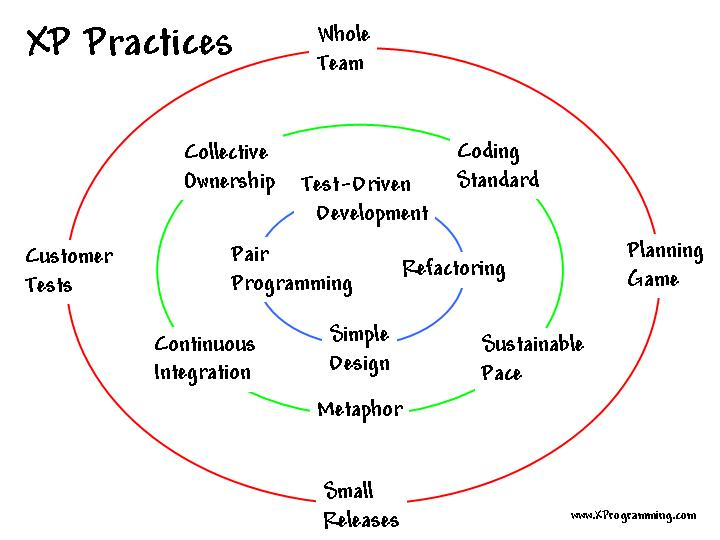
\includegraphics[width=0.8\textwidth]{images/xpCircles}
  \caption{Vorgehensweisen bei XP \cite{bib:xprogamming}}
  \label{fig:xppractices}
\end{figure}

\subsubsection{Planung}
Die Anforderungen an die Softwarelösung werden in sogenannten \emph{User Stories} festgehalten. Jede Story beschreibt eine Funktion, die der Kunde möchte. Eine solche User Story könnte wie folgt lauten:
\begin{quote}
Anzeige einer Druckvorschau beim Auswählen der Druckfunktion
\end{quote}
Danach wird ein Release-Plan erstellt. In der Regel werden alle drei Monate Releases veröffentlicht. Bei der Erstellung des Plans legen die Entwickler fest, welche User Story in welchem Release implementiert werden soll. Der Zeitraum zwischen zwei Releases wird wiederum in ein- bis drei-wöchigen Iterationen unterteilt. Zu Beginn jeder Iteration wählt der Kunde, die für ihn wichtigsten User Stories aus. Die Entwickler entwerfen, implementieren und testen die ausgewählten Stories innerhalb der Iteration. Am Ende jeder Iteration muss das Programm lauffähig sein, auch wenn noch wichtige Funktionen fehlen. 

\subsubsection{Management}
Auch für das Management eines Softwareprojekts sind bei XP klare Regeln definiert. Täglich gibt es ein Meeting, bei dem jeder Entwickler kurz sagt, was er am Vortag getan hat, was er heute tun wird und welche Probleme er sieht. Eine weitere wichtige Regel ist, dass ein Entwickler nicht länger arbeiten darf, als er auf unbefristete Zeit leisten kann. Normalerweise sind dies acht Stunden pro Tag. Überstunden sind nicht gern gesehen. Des Weiteren soll jeder Entwickler in den gesamten Prozess eingebunden sein und immer über den Gesamtstand der Projektes informiert sein. Außerdem sollen Entwickler immer wieder mit anderen Aufgaben betraut werden. Damit soll vermieden werden, dass sie den Anschluss zum technologischen Geschehen nicht verlieren. Aus dem selben Grund soll den Entwicklern auch genügend Freiraum gegeben werden, um auch während eines Projekts sich mit technischen Neuerungen zu befassen.

\subsubsection{Quellcodedesign}
Da im Gegensatz zu traditionellen Vorgehensmodellen die endgültige Architektur der Softwarelösung während der Programmierung noch nicht klar ist, sind beim Design einige Regeln zu beachten. Die wichtigste ist hier die Einfachheit. Der Quellcode ist so einfach wie möglich zu halten. Es sollen keine unnötigen Funktionen implementiert werden und es ist so zu programmieren, dass jeder aus dem Team den Quellcode verstehen kann. Des Weiteren soll immer wenn es sinnvoll ist, refactort werden.

\subsubsection{Testmanagement}
Bei Extreme Programming wird testgetrieben entwickelt. Das heißt, es werden zuerst die Unit-Tests einer Funktion geschrieben. Erst danach darf die Funktion selbst geschrieben. Diese Art der Programmierung zwingt den Programmierer zu einer genaueren Überlegung, was die Funktion erledigen soll und welche Grenzfälle dabei auftreten können. Und dabei stellt das \emph{Test First} genannte Prinzip gleichzeitig sicher, dass es eine komplette Testabdeckung gibt. Die Unit-Tests werden mehrmals täglich ausgeführt. Zur weiteren Verbesserung der Qualität werden die Änderungen der Entwickler mehrfach am Tag in die gemeinsame Quellcodebasis integriert. Dieser Integrationstest stellt sicher, dass die einzelnen Teilkomponenten korrekt miteinander arbeiten. Noch eine Stufe abstrakter ist der \emph{Acceptance Test}. Dies ist ein Black-Box-Test, der nach jeder Iteration vom Kunde durchgeführt wird. Jeder Fehler, der vom Kunde gemeldet wird, muss mit einem Unit-Test abgedeckt werden um ihn zukünftig zu vermeiden.

\subsubsection{Programmierung}
Die auffälligste Unterscheidung von XP zu traditionellen Vorgehensmodellen ist das \emph{Pair Programming}. Es sitzen immer zwei Entwickler vor einem Rechner und einer Tastatur und programmieren gemeinsam. Dabei wechseln sie sich regelmäßig ab beim Schreiben des Codes. Dies soll bei geringem Zeitverlust eine starke Qualitätssteigerung mit sich bringen. Weniger auffällig, aber trotzdem wichtig ist die Regel, dass jeder Entwickler das Recht hat jede Codezeile des Projektes zu ändern. Das heißt, wenn ihm Fehler oder Unstimmigkeiten auffallen, kann er diese gleich beheben. 

\subsection{Scrum}
\label{ch:scrum}
Laut einer Studie von 2010 von \emph{Forrester Research} ist Scrum die verbreitetste agile Methode. So verwendeten ca. 11 \% der befragten IT-Fach\-kräfte das wohl bekannteste agile Vorgehensmodell. \cite{bib:ane} Scrum bietet deutlich weniger Regeln als Extreme Programming und gilt somit als verhältnismäßig leicht einzusetzen. Jedoch muss dabei beachtet werden, dass lediglich Vorgaben für die Planung und das Management eines Softwareprojekts gestellt werden. 

\subsubsection{Rollenverteilung}
Im Zentrum von Scrum ein hochmotiviertes und selbstgesteuertes Entwicklerteam. Die Rollenverteilung von klassischen Vorgehensmodellen wird grundlegend verändert. Der Produktmanager wird zum Product Owner. Der Teamleiter wird zum Scrum Master. Und das Team, zu dem alle Entwickler gehören, bekommt deutlich mehr Verantwortung.

\begin{description}
\item{Product Owner}\\
Er bringt die Produktvision mit sich und ist verantwortlich für das Produkt. Dabei definiert er die Anforderungen, priorisiert sie und kontrolliert die Ergebnisse. Zusätzlich behält er das Budget und die Wirtschaftlichkeit im Blick. Wichtig: Der Product Owner gibt dem Team keine Zeitvorgaben.

\item{Scrum Master}\\
Der Scrum Master sorgt für die Einhaltung des Entwicklungsprozesses und den Scrum-Regeln. Hierzu schützt er das Team auch vor Störungen von außen und beseitigt organisatorische Probleme. Wichtig: Der Scrum Master vergibt keine Aufgaben.

\item{Team}\\
Das Team steht im Mittelpunkt des Entwicklungsprozesses. Es entscheidet selbst wann es welche Aufgaben erledigt. Verantwortung übernimmt das Team für das Zeit-, Qualitäts- und Dokumentationsmanagement.
\end{description}

\subsubsection{Prozess}
Die Abbildung \ref{fig:scrum} stellt das Vorgehen bei Scrum dar. Zu Beginn des Projekts stellt der Product Owner das \emph{Product Backlog} auf, in dem die Anforderungen des Produkts mit User Stories beschrieben werden. Das Product Backlog kann jederzeit vom Product Owner mit weiteren Anforderungen erweitert. Jede Anforderung bekommt vom Product Owner eine Priorität, die sich auch im Laufe des Projekts verändern kann. Das priorisierte Product Backlog stellt der Product Owner im \emph{Sprint Planning Meeting} dem Team vor. Beim Sprint Planning Meeting wählt das Team so viele User Stories aus dem Product Backlog aus, wie es denkt während der nächsten Iteration (\emph{Sprint} abarbeiten zu können. Die User Stories teilt das Team in einzelne Aufgaben auf und hält sie im \emph{Sprint Backlog} fest. Das Sprint Backlog darf während einer Iteration nicht verändert werden.

\begin{figure}[h]
  \centering
  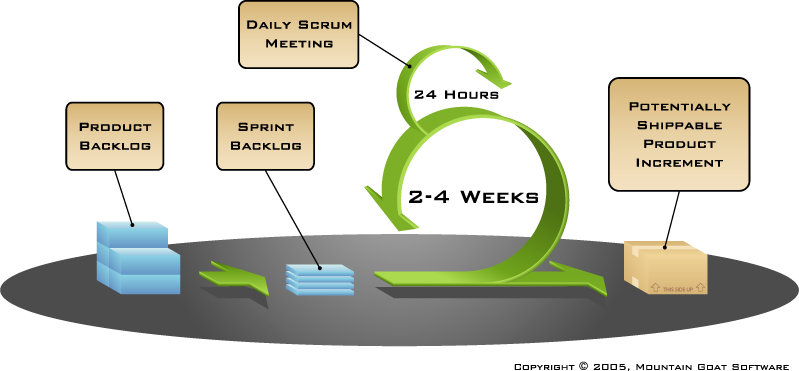
\includegraphics[width=1\textwidth]{images/scrum}
  \caption{Prozessüberblick bei Scrum \cite{bib:mountaingoat}}
  \label{fig:scrum}
\end{figure}

Nach dem Meeting beginnt der Sprint. Ein Sprint stellt eine Iteration von zwei bis vier Wochen dar und wird immer wieder durchlaufen. Während des Sprints findet täglich ein \emph{Daily Scrum Meeting} statt an dem das Team und der Scrum Master teilnehmen. Dieses ist gleich aufgebaut wie das tägliche Meeting beim Extreme Progamming. Die Dauer des Meetings legt der Scrum Master in der Regel auf 15 Minuten fest und hält dies auch ein. Jeder Teilnehmer bespricht kurz die folgenden drei Dinge: 
\begin{itemize}
  \item Was habe ich gestern gemacht? 
  \item Was steht heute auf dem Plan? 
  \item Und welche Probleme habe sehe ich?
\end{itemize}
Im Sprint Backlog wird der tägliche Fortschritt festgehalten. Dadurch entsteht ein immer aktuelles Burn-Down Diagramm (Abbildung \ref{fig:burndown}), das den Fortschritt des Sprints übersichtlich darstellt. 

\begin{figure}[h]
  \centering
  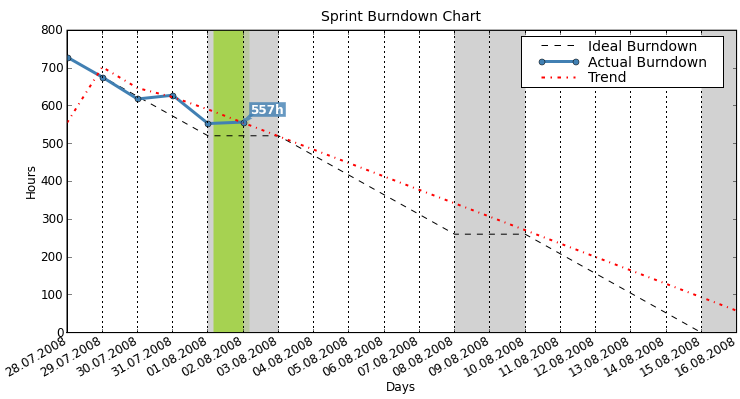
\includegraphics[width=0.8\textwidth]{images/burndown}
  \caption{Burn-Down Diagramm eines Sprints \cite{bib:agilo}}
  \label{fig:burndown}
\end{figure}

Am Ende des Sprints muss eine lauffähige Version des Programms verfügbar sein, die dem Product Owner im \emph{Sprint Review Meeting} präsentiert wird. Zusätzlich gibt es noch das \emph{Sprint Retrospectiv Meeting}, an dem über den vergangen Sprint reflektiert wird um über Veränderungen eine Verbesserung des Prozesses zu erzielen.

\subsubsection{Scrum Anti-Pattern}
Marion Eickmann schreibt, dass Scrum nur dann funktioniert, wenn auch alle Beteiligten sich an die Regeln halten: ``Alle Beteiligten müssen sich an das neue Vorgehen gewöhnen und sind unsicher was zu tun ist, wenn Unerwartetes geschieht. Solche Schwierigkeiten führen häufig dazu, `bekannte' Mechanismen `nur für den Fall' anzuwenden, statt das Problem nach Scrum-Art zu lösen.'' \cite[S. 84]{bib:ix2010}. So führt sie in ihrem Artikel mehrere bekannte Scrum Anti-Pattern auf, die es gilt zu vermeiden. Die wichtigsten seien hier aufgezählt:
\begin{itemize}
  \item Der Scrum Master weist Tasks zu und zerstört so das sich selbst steuernde und organisierende Team
  \item Der Sprint wird von außen gestört. Es werden neue Aufgaben eingefügt oder Änderungen an den gewählten (committed) user Stories vorgenommen.
  \item Es finden keine Review Meeting statt
  \item Es findet keine Retrospective statt
  \item Es gibt keine regelmäßigen Daily Standup Meetings
  \item Der Product Owner hat keine ausreichende Kompetenz und nimmt seine Rolle nicht war
  \item Meetings sind nicht Time-Boxed
  \item Statt Funktionen werden Aktivitäten erfasst
\end{itemize} 

\subsection{Software Kaban}

